%!TEX root = ../main.tex
% =============================================================
%  CAPÍTULO 5 — JUSTIFICACIÓN ECONÓMICA (Entrega 5 · 15 % · 15/9)
% =============================================================

\chapter{Justificación económica}\label{cap:economica}

\begin{guia}[Guía de la cátedra: qué se evalúa en este capítulo]
Es el capítulo de mayor peso individual (15\,\%). Se evalúa como una
evaluación de proyectos de inversión:
\begin{enumerate}
    \item \textbf{Análisis de mercado y competidores}: tamaño, segmentos,
          precios de referencia.
    \item \textbf{Modelo de negocio}: B2B, B2C, B2G o interno; niveles de
          precio y fuentes de ingreso.
    \item \textbf{Inversión inicial} desglosada por rol y tiempo, más
          infraestructura.
    \item \textbf{Costos operativos} recurrentes.
    \item \textbf{Escenarios} pesimista, base y optimista, con flujo de caja
          proyectado a 3 a 5 años.
    \item \textbf{Indicadores}: \gls{van}, \gls{tir} y período de repago,
          con una tasa de descuento construida y justificada con fuentes.
    \item \textbf{Supuestos y restricciones} explícitos.
\end{enumerate}
Todo número con su origen: cotización, tarifa pública, estadística
citada o estimación propia declarada como tal.
\end{guia}

\section{Escenario de comercialización}\label{sec:n5.1}

El proyecto se evalúa bajo un modelo de suscripción, distribuido como aplicación web en la que el análisis se ejecuta en el navegador del usuario, complementada por una herramienta de línea de comandos (CLI) integrable en pipelines de integración y despliegue continuos. El abono mensual se fijó en USD 8 por usuario, equivalente a USD 96 anuales bajo facturación anualizada.

\subsection{Suscripción frente a licencia perpetua}\label{sec:n5.1.1}

La elección de la suscripción responde a dos motivos, uno financiero y otro técnico:

\paragraph{Recurrencia frente a esfuerzo continuo de reposición.} La suscripción genera un flujo de fondos predecible, en el que los usuarios captados continúan aportando en los ejercicios posteriores mientras utilicen la herramienta. Un esquema de licencia única obligaría a captar un volumen equivalente de clientes nuevos cada año solo para sostener el nivel de ingresos. A ello se suma que una herramienta de análisis estático demanda actualización periódica de reglas para cubrir nuevos patrones de vulnerabilidad y versiones de librerías, tarea de mantenimiento que se financia de manera natural con ingresos periódicos.

\paragraph{Inconsistencia de precios relativos.} A USD 8 por mes, un cliente iguala en cinco meses el valor típico de una licencia perpetua individual, estimada en torno a USD 50. Ofrecer ambas modalidades en paralelo a esos valores generaría arbitraje en contra de la suscripción, o exigiría fijar la licencia perpetua a un precio fuera de mercado.

\subsection{Público objetivo}\label{sec:n5.1.2}

El producto se orienta a tres segmentos:

\paragraph{Desarrolladores independientes.} Programadores de JavaScript y TypeScript, en entornos Node.js, Express y React, que necesitan auditar código fuente localmente para prevenir inyecciones SQL (CWE-89), inyecciones de comandos del sistema operativo (CWE-78) y Cross-Site Scripting (CWE-79) antes de enviar cambios al repositorio.

\paragraph{Equipos de desarrollo en PyMEs y empresas de reciente creación.} Grupos de tres a quince desarrolladores que buscan implementar prácticas de seguridad temprana sin la carga presupuestaria ni la infraestructura que requieren las suites corporativas.

\paragraph{Consultores de aseguramiento de calidad y seguridad de aplicaciones.} Profesionales que realizan auditorías puntuales sobre código de terceros.

\subsection{Relación entre público y precio}\label{sec:n5.1.3}

Las soluciones corporativas consolidadas del mercado operan con contratos anuales de miles de dólares y requieren servidores dedicados. Frente a ellas, USD 8 mensuales equivalen aproximadamente a una hora de desarrollo junior en Argentina, según la tarifa de referencia adoptada en la sección~\ref{sec:n5.2}. Ese orden de magnitud elimina la barrera de entrada para un profesional independiente o para el responsable técnico de una empresa pequeña, dado que la decisión de compra no requiere aprobaciones presupuestarias complejas.

\subsection{Dimensionamiento del mercado}\label{sec:n5.1.4}

\paragraph{Mercado total direccionable.} El relevamiento global de SlashData (State of the Developer Nation) y el reporte anual GitHub Octoverse ubican a JavaScript y TypeScript de forma constante a la cabeza del ranking de adopción, con una base mundial superior a los veinte millones de programadores. La distribución como aplicación web, accesible desde el navegador sin instalación, junto con la publicación de la herramienta de línea de comandos en el registro de paquetes npm, canal habitual de las herramientas de desarrollo del ecosistema JavaScript, permite alcanzar esa base sin intermediarios comerciales.

\paragraph{Mercado disponible regional.} Para dimensionar el mercado local se parte del dato publicado por el Observatorio Permanente de la Industria del Software y Servicios Informáticos (OPSSI) de CESSI, que registra 162.598 puestos de trabajo formales en el sector al primer trimestre de 2026. Dado que esa cifra comprende la totalidad de las funciones de las empresas —gestión, soporte, infraestructura y administración—, la proporción estrictamente técnica se estima a partir de los relevamientos de la Encuesta de Sueldos de Sysarmy, en los que los roles de desarrollo concentran entre el 50 \% y el 60 \% del personal técnico. Asumiendo de forma conservadora que entre un 35 \% y un 50 \% de ese personal de desarrollo trabaja sobre aplicaciones web en el ecosistema JavaScript/TypeScript, el mercado accesible local se ubica en un orden de entre 28.000 y 49.000 desarrolladores.

\paragraph{Mercado objetivo.} La proyección contempla alcanzar 20 usuarios en el primer año y escalar gradualmente hasta 300 usuarios activos en el quinto. Sobre el mercado accesible estimado, esos 300 suscriptores representan una cuota de penetración de entre el 0,6 \% y el 1,1 \%, lo que muestra que la factibilidad del flujo no descansa en metas de captación desmedidas.

\section{Inversión inicial}\label{sec:n5.2}

La inversión comprende las horas de ingeniería y los desembolsos requeridos para transformar el prototipo funcional en un producto comercializable: la aplicación web con cobro de suscripciones y acceso controlado por licencia.

\subsection{Supuestos de la estimación de horas}\label{sec:n5.2.1}

Los parámetros de dedicación correspondientes a la fase de prototipo y a las tareas pendientes hasta el lanzamiento se resumen en la tabla~\ref{tab:supuestos-horas}.

\begin{table}[H]
    \centering
    \caption{Supuestos de estimación de horas de desarrollo}
    \label{tab:supuestos-horas}
    \small
    \begin{tabularx}{\textwidth}{L L}
        \toprule
        \tb{Parámetro} & \tb{Valor adoptado} \\
        \midrule
        Período de desarrollo del prototipo & Mediados de junio a mediados de septiembre de 2026 (13 semanas) \\
        Días dedicados por semana & 3 a 4 días (promedio: 3,5) \\
        Horas diarias de trabajo & 4 a 5 horas (promedio: 4,5) \\
        Carga semanal estimada & $\approx$ 15,75 horas \\
        Horas insumidas en el prototipo & $\approx$ 205 horas (rango representativo: 156 a 260) \\
        Horas adicionales hasta producto comercializable & 400 horas (cobro de suscripciones y emisión de licencias, control de acceso en la aplicación web, publicación de la herramienta de línea de comandos en npm, documentación y pruebas con usuarios) \\
        \bottomrule
    \end{tabularx}
\end{table}

\subsection{Determinación del valor hora}\label{sec:n5.2.2}

Se adoptó un valor de USD 8 por hora como costo total para el empleador. La cifra se construye en tres pasos. La Encuesta de Sueldos 2026.01 de Sysarmy, analizada por OpenQube, reporta para la categoría Junior en Argentina una mediana salarial bruta de ARS 1.538.500 mensuales; sobre un estándar de 160 horas laborales mensuales, ello equivale a ARS 9.616 por hora de salario bruto. A dicho valor corresponde adicionar las contribuciones patronales y cargas sociales, que en el régimen argentino incrementan el costo laboral en aproximadamente un 25 \% respecto del salario bruto, con lo que el costo por hora asciende a ARS 12.020. Convertido al tipo de cambio mayorista de referencia indicado en la sección~\ref{sec:n5.4}, el valor resultante se ubica en el orden de USD 8 por hora.

Se emplea el costo total para el empleador, y no el salario bruto percibido, por tratarse de la magnitud que refleja el verdadero consumo de recursos que implica cada hora de desarrollo.

\subsection{Composición de la inversión inicial}\label{sec:n5.2.3}

En la tabla~\ref{tab:inversion} se detallan las erogaciones previstas para el Año 0.

\begin{table}[H]
    \centering
    \caption{Presupuesto de inversión inicial (Año 0)}
    \label{tab:inversion}
    \small
    \begin{tabularx}{\textwidth}{L L r}
        \toprule
        \tb{Concepto} & \tb{Cálculo} & \tb{Importe (USD)} \\
        \midrule
        Desarrollo del prototipo & 205 h $\times$ USD 8 & 1.640 \\
        Desarrollo hasta versión comercializable & 400 h $\times$ USD 8 & 3.200 \\
        Marketing y lanzamiento inicial & Sitio informativo, registro y difusión & 500 \\
        Licencias de software & Pila tecnológica de código abierto & 0 \\
        Hardware y equipamiento & Equipo informático propio disponible & 0 \\
        Infraestructura de servidores & Plan gratuito de Vercel durante el desarrollo, sin uso comercial & 0 \\
        Total inversión inicial (Año 0) &  & 5.340 \\
        \bottomrule
    \end{tabularx}
\end{table}

\section{Costos post-proyecto}\label{sec:n5.3}

Los costos operativos anuales necesarios para sostener la herramienta durante el horizonte de cinco años comprenden tres componentes.

El primero corresponde al mantenimiento técnico y al soporte. Se estiman seis horas mensuales destinadas a la atención de incidencias, la corrección de errores y la actualización del catálogo de reglas, valorizadas al costo horario adoptado, lo que arroja un costo anual fijo de USD 576.

El segundo corresponde al alojamiento y al dominio. La aplicación web se publica en Vercel, cuyo plan gratuito se limita al uso personal no comercial; la comercialización exige el plan Pro, con un abono fijo de USD 20 mensuales (USD 240 anuales) que incluye 1 TB mensual de transferencia de datos, volumen holgado para una aplicación estática cuyo análisis se ejecuta en el navegador. La validación de las licencias se resuelve con una función de servidor de consumo marginal, cuyo excedente sobre el uso incluido en el plan se factura a USD 0,60 por millón de invocaciones. La renovación del dominio .com cuesta USD 11,25 anuales en el registrador de Vercel, redondeados a USD 11.

El tercero corresponde a las comisiones de cobro. El cobro de las suscripciones y la emisión de licencias se delegan en Lemon Squeezy, que actúa como comerciante registrado (merchant of record): procesa los pagos, liquida los impuestos al consumo de cada país y emite claves de licencia que vencen junto con la suscripción, por lo que la aplicación no necesita administrar cuentas de usuario propias. Su comisión es del 5 \% más USD 0,50 por transacción, sin cargo mensual; Paddle, alternativa equivalente, aplica la misma tarifa. Con facturación anual, cada suscriptor genera una transacción de USD 96 y una comisión de USD 5,30, de modo que este rubro crece con la base de usuarios.

\begin{table}[H]
    \centering
    \caption{Costos operativos anuales post-proyecto, en dólares (Años 1 a 5)}
    \label{tab:costos-operativos}
    \small
    \begin{tabularx}{\textwidth}{L r r r r r}
        \toprule
        \tb{Rubro} & \tb{Año 1} & \tb{Año 2} & \tb{Año 3} & \tb{Año 4} & \tb{Año 5} \\
        \midrule
        Mantenimiento y soporte & 576 & 576 & 576 & 576 & 576 \\
        Alojamiento (Vercel Pro) & 240 & 240 & 240 & 240 & 240 \\
        Dominio & 11 & 11 & 11 & 11 & 11 \\
        Comisiones de cobro & 106 & 318 & 636 & 1.060 & 1.590 \\
        Costo operativo total anual & 933 & 1.145 & 1.463 & 1.887 & 2.417 \\
        \bottomrule
    \end{tabularx}
\end{table}

\section{Flujo de fondos proyectado}\label{sec:n5.4}

\subsection{Supuestos del flujo}\label{sec:n5.4.1}

\paragraph{Moneda de cuenta.} La totalidad del flujo se expresa en dólares estadounidenses, con el objeto de aislar la proyección del efecto de la inflación en moneda local. Como referencia para los costos originados en pesos se tomó el tipo de cambio mayorista de la Comunicación «A» 3500 del Banco Central de la República Argentina, que al 11 de septiembre de 2026 se ubicó en ARS 1.509,91 por dólar.

\paragraph{Ingreso por usuario.} Cada suscriptor activo abona USD 96 por año en un único pago anual, equivalentes a USD 8 mensuales. Los impuestos al consumo que liquida el procesador de pagos se suman al precio y no forman parte del ingreso.

\paragraph{Adopción progresiva.} 20 usuarios en el primer año, 60 en el segundo, 120 en el tercero, 200 en el cuarto y 300 en el quinto.

\paragraph{Cómputo temporal.} La inversión se efectúa en el momento inicial (Año 0), mientras que los cobros y los costos operativos se imputan al cierre de cada ejercicio anual.

\begin{table}[H]
    \centering
    \caption{Flujo de fondos proyectado, en dólares (Años 0 a 5)}
    \label{tab:flujo-caja}
    \small
    \begin{tabularx}{\textwidth}{l r r r r L}
        \toprule
        \tb{Año} & \tb{Usuarios} & \tb{Ingresos} & \tb{Costos} & \tb{Flujo neto} & \tb{Flujo acumulado} \\
        \midrule
        0 & — & — & — & $-$5.340 & $-$5.340 \\
        1 & 20 & 1.920 & $-$933 & 987 & $-$4.353 \\
        2 & 60 & 5.760 & $-$1.145 & 4.615 & 262 \\
        3 & 120 & 11.520 & $-$1.463 & 10.057 & 10.319 \\
        4 & 200 & 19.200 & $-$1.887 & 17.313 & 27.632 \\
        5 & 300 & 28.800 & $-$2.417 & 26.383 & 54.015 \\
        Total &  & 67.200 & $-$7.845 & 54.015 &  \\
        \bottomrule
    \end{tabularx}
\end{table}

La figura~\ref{fig:flujo-fondos} representa el mismo flujo: las barras corresponden al flujo neto de cada año y la línea, al acumulado, que cruza el cero a los 1,94 años.

\begin{figure}[H]
    \centering
    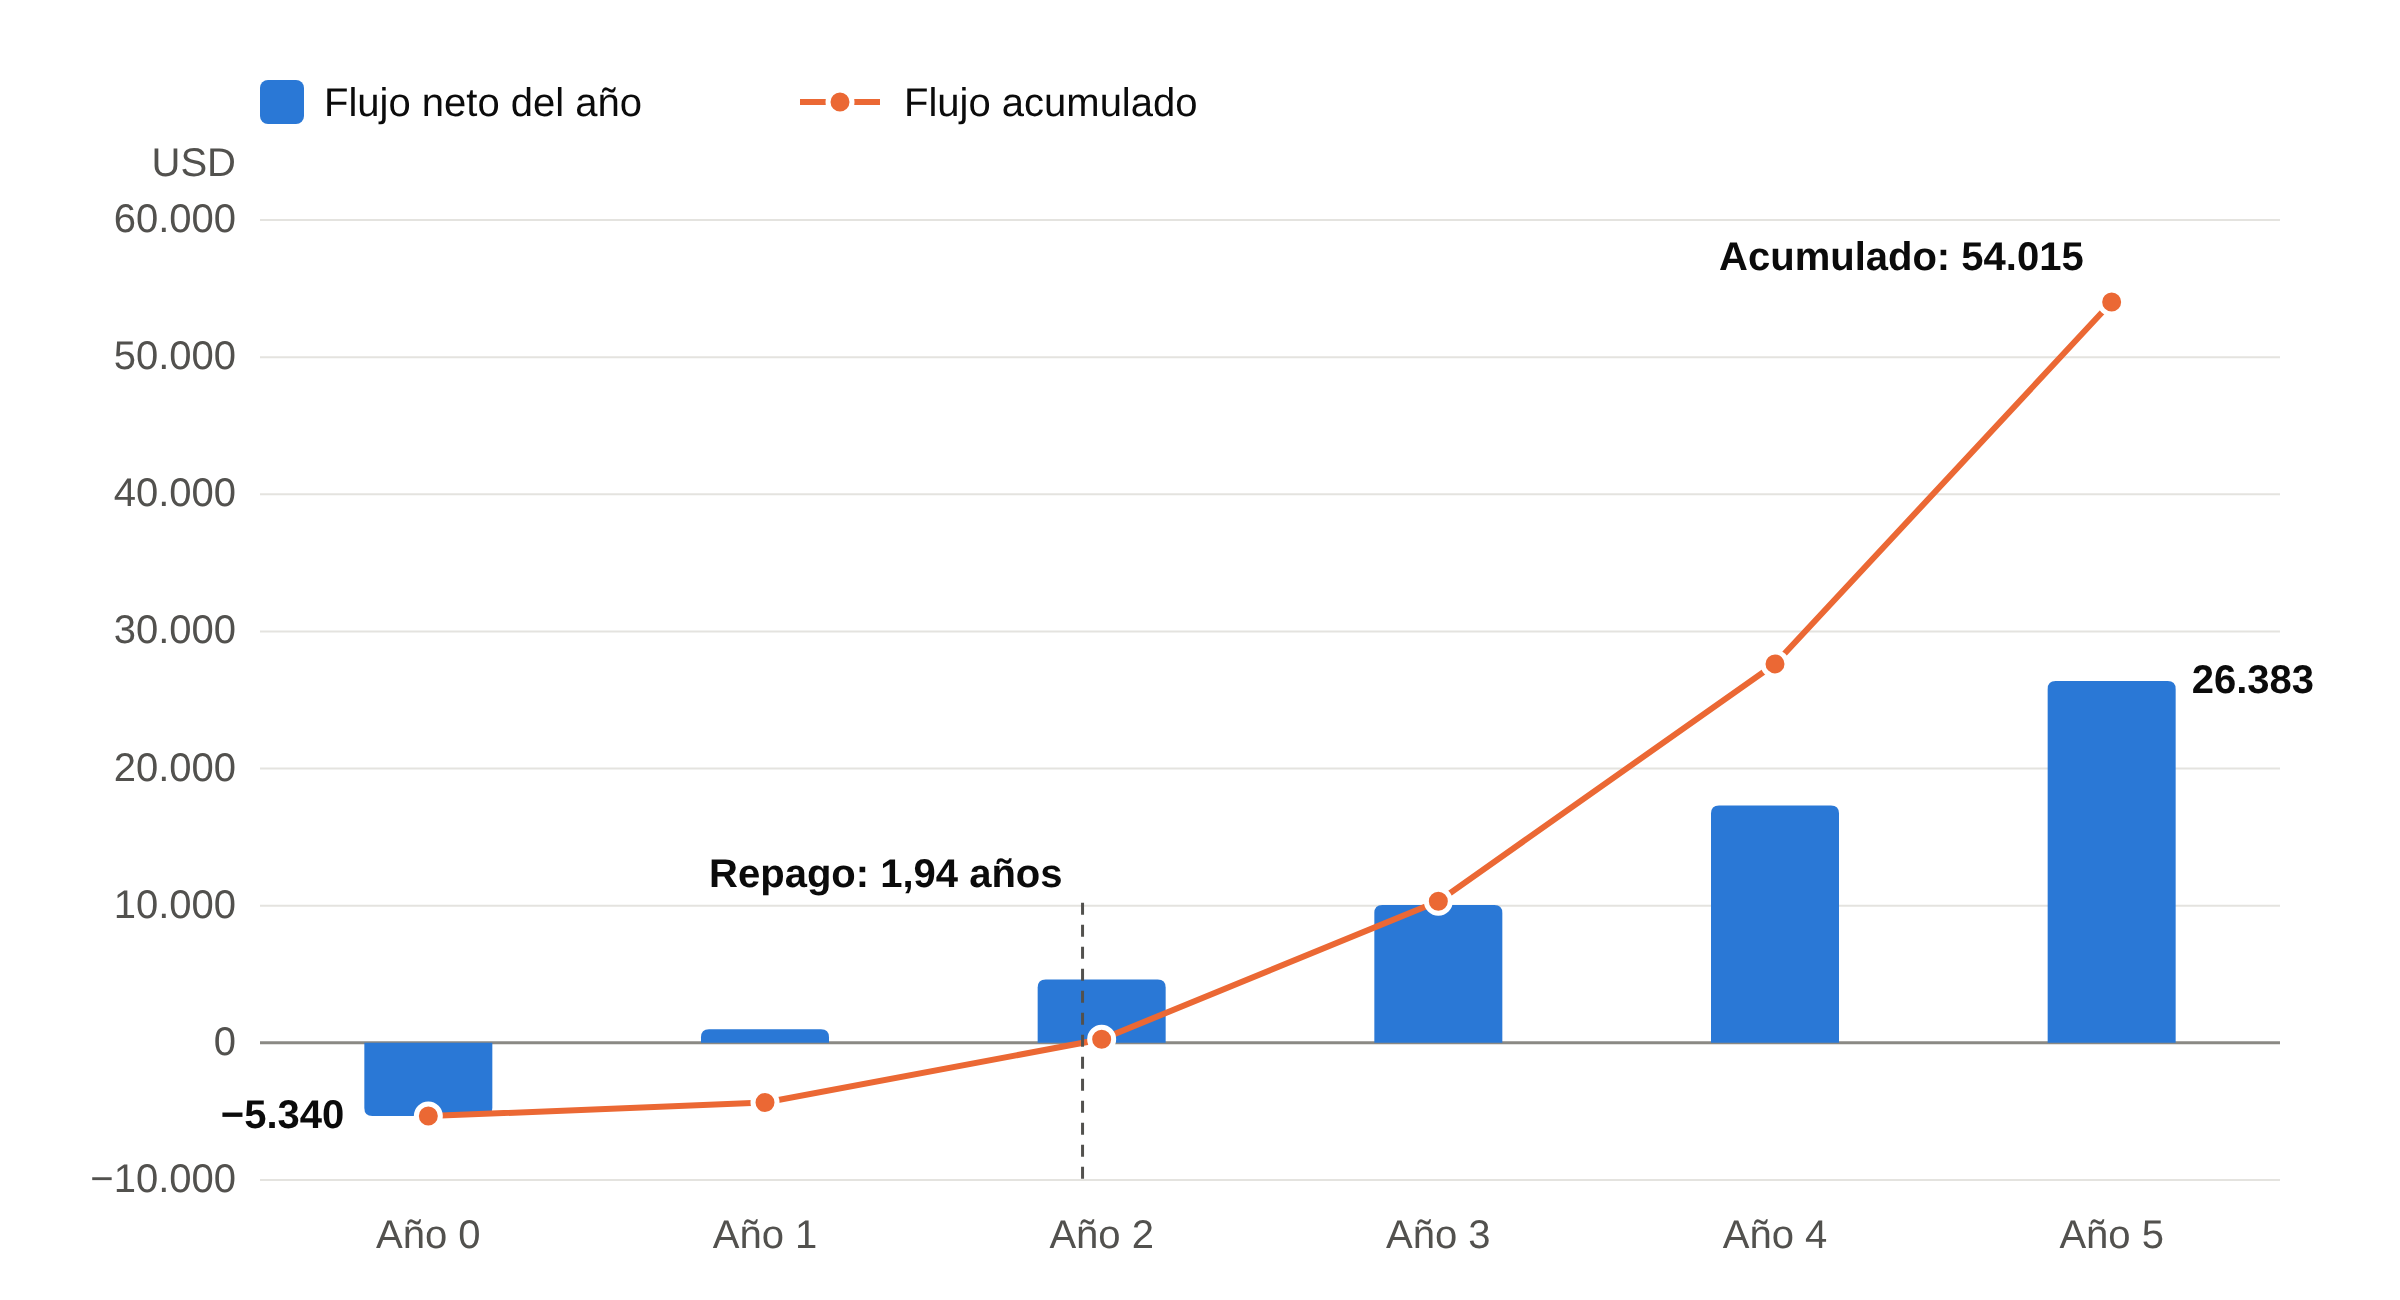
\includegraphics[width=0.9\textwidth]{figuras/flujo-fondos.png}
    \caption{Flujo de fondos neto y acumulado, en dólares (Años 0 a 5). El acumulado se vuelve positivo a los 1,94 años}
    \label{fig:flujo-fondos}
\end{figure}

\section{Tasa de descuento}\label{sec:n5.5}

Se adopta una tasa de descuento del 20 \% anual en dólares. La tasa integra los tres componentes conceptuales del costo de capital.

\paragraph{Costo de oportunidad del capital.} El rendimiento de un activo libre de riesgo en dólares, representado por los bonos del Tesoro de los Estados Unidos a diez años, se ubica en torno al 3,8 \% y el 4,3 \% anual. Una inversión diversificada de mercado en el índice S\&P 500 promedia históricamente un retorno nominal del 9 \% al 10 \% anual en moneda dura.

\paragraph{Inflación de la moneda de evaluación.} Al confeccionar el flujo en dólares se neutraliza la inflación local en pesos, e incide únicamente la meta de inflación de largo plazo del Comité Federal de Mercado Abierto de la Reserva Federal de los Estados Unidos, fijada en el 2 \% anual.

\paragraph{Riesgo específico de etapa temprana.} El proyecto consiste en una herramienta de software que parte sin antecedentes comerciales ni base instalada. La literatura de finanzas corporativas aplicada a la valuación de emprendimientos tecnológicos —en particular las bases de datos de costo de capital de Aswath Damodaran, de la Stern School of Business de la Universidad de Nueva York, y los rangos de referencia empleados para inversiones en etapa semilla— establece tasas de corte de entre el 18 \% y el 25 \% anual en dólares para proyectos tecnológicos incipientes.

Una tasa del 20 \% anual reconoce el costo de oportunidad del capital y remunera de manera adecuada la prima de riesgo asociada a un desarrollo sin tracción comercial previa.

\section{Indicadores financieros}\label{sec:n5.6}

A partir del flujo de fondos de la tabla~\ref{tab:flujo-caja}, y aplicando la tasa de descuento del 20 \%, se obtuvieron los indicadores que expone la tabla~\ref{tab:indicadores-financieros}.

\begin{table}[H]
    \centering
    \caption{Resultados de los indicadores financieros}
    \label{tab:indicadores-financieros}
    \small
    \begin{tabularx}{\textwidth}{l l L l}
        \toprule
        \tb{Indicador} & \tb{Resultado} & \tb{Criterio de decisión} & \tb{Conclusión} \\
        \midrule
        Período de repago simple & 1,94 años & Menor al horizonte de evaluación & Aceptable \\
        Período de repago descontado & 2,23 años & Menor al horizonte de evaluación & Aceptable \\
        Valor Actual Neto (20 \%) & USD 23.459 & VAN > 0 & Crea valor \\
        Tasa Interna de Retorno & 93,5 \% & TIR > 20 \% & Supera el mínimo exigido \\
        \bottomrule
    \end{tabularx}
\end{table}

\subsection{Lectura de los indicadores}\label{sec:n5.6.1}

\paragraph{Repago simple (1,94 años).} El proyecto recupera la inversión inicial durante el segundo año de operación, únicamente con sus flujos netos de caja.

\paragraph{Repago descontado (2,23 años).} Medido en dinero de hoy, el recupero se posterga aproximadamente tres meses y medio respecto del cálculo sin descontar; esa diferencia constituye el precio del tiempo.

\paragraph{Valor Actual Neto (USD 23.459).} El proyecto devuelve la inversión, remunera el 20 \% anual exigido y deja un excedente cercano a los USD 23.500, medidos en dinero de hoy.

\paragraph{Tasa Interna de Retorno (93,5 \%).} El rendimiento anual implícito supera ampliamente la tasa exigida; la tasa de corte podría elevarse hasta ese valor antes de que el proyecto dejara de convenir.

\section{Análisis de sensibilidad y escenarios}\label{sec:n5.7}

\subsection{Sensibilidad del Valor Actual Neto a la tasa de descuento}\label{sec:n5.7.1}

En la tabla~\ref{tab:sensibilidad-tasa} se evalúa la respuesta del Valor Actual Neto ante incrementos sucesivos de la tasa de corte exigida, entre el 10 \% y el 40 \% anual.

\begin{table}[H]
    \centering
    \caption{Sensibilidad del Valor Actual Neto frente a variaciones en la tasa de descuento}
    \label{tab:sensibilidad-tasa}
    \small
    \begin{tabularx}{\textwidth}{l L}
        \toprule
        \tb{Tasa de descuento} & \tb{Valor Actual Neto (USD)} \\
        \midrule
        10 \% & 35.134 \\
        15 \% & 28.636 \\
        20 \% (tasa base) & 23.459 \\
        25 \% & 19.289 \\
        30 \% & 15.895 \\
        40 \% & 10.797 \\
        \bottomrule
    \end{tabularx}
\end{table}

El Valor Actual Neto se mantiene positivo aun elevando la tasa de corte al 40 \%, lo que verifica que la viabilidad del proyecto no depende de una tasa adoptada de forma arbitraria.

\begin{figure}[H]
    \centering
    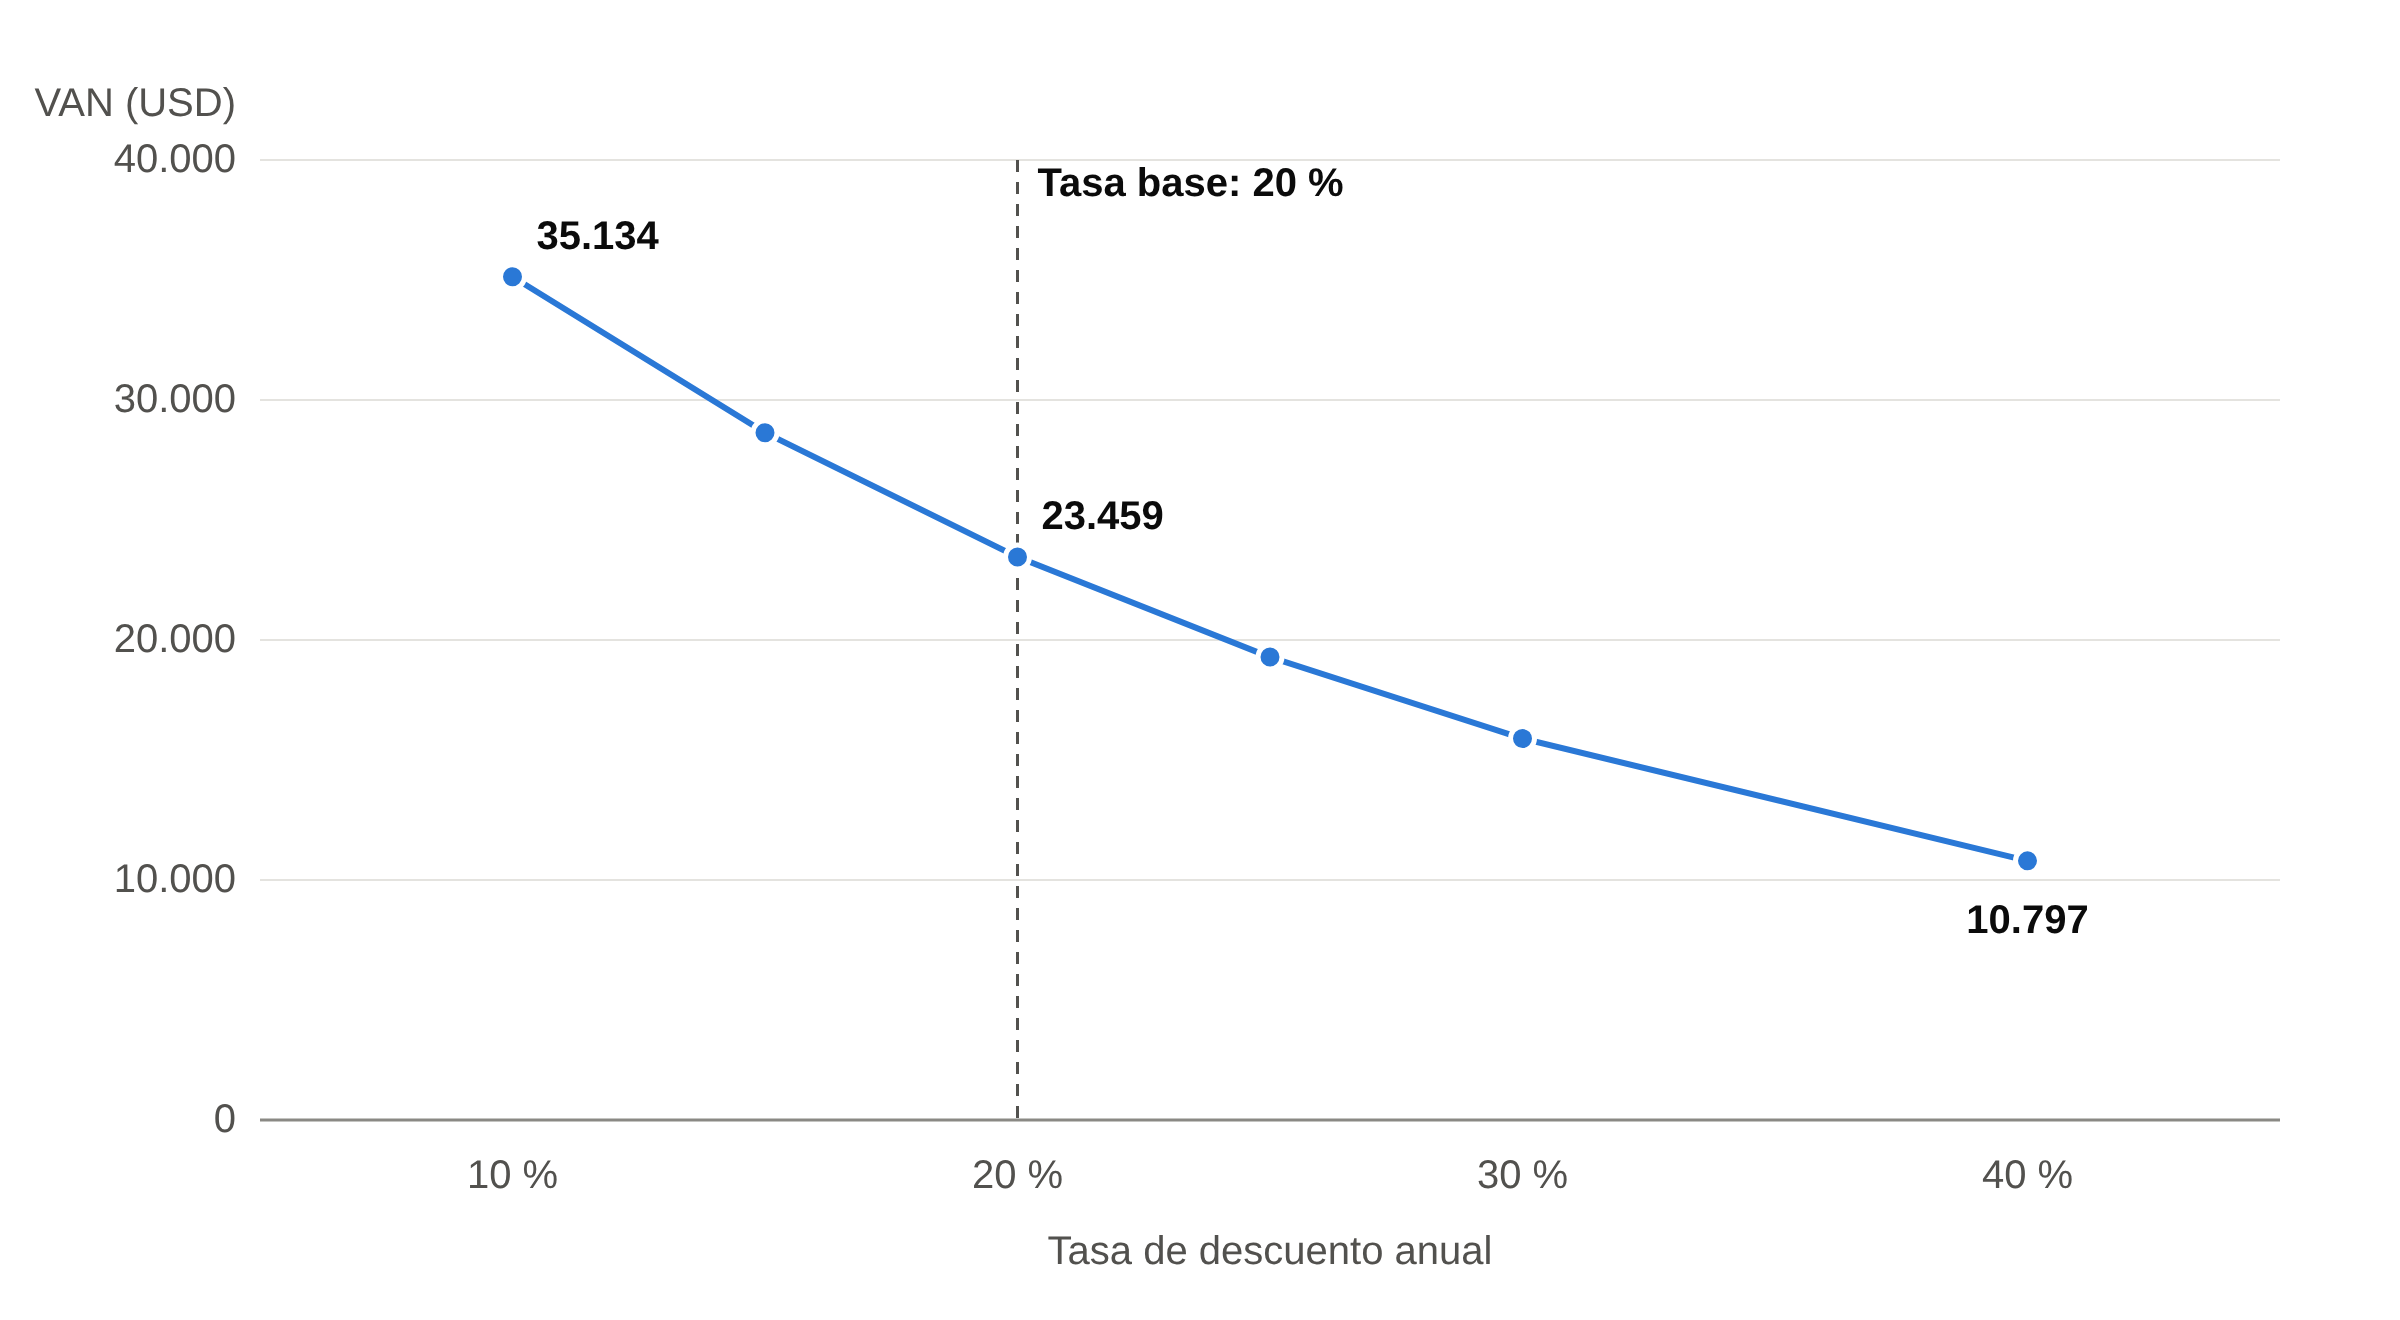
\includegraphics[width=0.9\textwidth]{figuras/van-tasa.png}
    \caption{Valor Actual Neto según la tasa de descuento anual}
    \label{fig:van-tasa}
\end{figure}

\subsection{Escenarios de adopción}\label{sec:n5.7.2}

Siendo la adopción de usuarios la variable de mayor dispersión, la tabla~\ref{tab:escenarios} modela tres situaciones: pesimista, con la mitad de los usuarios proyectados; base, con la proyección original; y optimista, con un 50 \% adicional.

\begin{table}[H]
    \centering
    \caption{Evaluación de escenarios sobre la base de usuarios}
    \label{tab:escenarios}
    \small
    \begin{tabularx}{\textwidth}{l L r r}
        \toprule
        \tb{Escenario} & \tb{Supuesto de usuarios} & \tb{VAN (USD)} & \tb{TIR} \\
        \midrule
        Pesimista & Mitad de los usuarios proyectados (10 a 150) & 7.823 & 51,7 \% \\
        Base & Proyección original adoptada (20 a 300) & 23.459 & 93,5 \% \\
        Optimista & 50 \% adicional sobre la base (30 a 450) & 39.096 & 125,5 \% \\
        \bottomrule
    \end{tabularx}
\end{table}

En el escenario pesimista, captando únicamente la mitad de los usuarios proyectados, el Valor Actual Neto resulta positivo en USD 7.823 y la Tasa Interna de Retorno alcanza el 51,7 \%, superando por 31,7 puntos porcentuales la tasa mínima exigida. El proyecto cuenta, por lo tanto, con margen para absorber desvíos en la captación sin comprometer su conveniencia financiera.

\section{Conclusión}\label{sec:n5.8}

El análisis muestra que el proyecto resulta viable desde el punto de vista económico: los cuatro indicadores calculados señalan rentabilidad positiva dentro del horizonte de cinco años. No obstante, esa viabilidad queda supeditada a condiciones concretas que corresponde declarar.

\subsection{Condición crítica}\label{sec:n5.8.1}

La variable determinante es la captación de usuarios. La inversión de capital es reducida y los costos operativos resultan bajos gracias a que el análisis se ejecuta en el navegador de cada usuario y el servidor solo entrega archivos estáticos. En consecuencia, el riesgo del proyecto no reside en la estructura de costos sino, de manera prácticamente exclusiva, en alcanzar la masa crítica inicial de suscriptores.

\subsection{Magnitud de la Tasa Interna de Retorno}\label{sec:n5.8.2}

El valor obtenido para la Tasa Interna de Retorno responde a la naturaleza económica de los productos de software: una vez cubiertas las horas fijas de desarrollo, el costo marginal de atender a un suscriptor adicional resulta prácticamente nulo. La magnitud del indicador debe interpretarse en ese marco y no como una expectativa de rentabilidad garantizada.

\subsection{Limitaciones del modelo}\label{sec:n5.8.3}

La evaluación incorpora tres simplificaciones que conviene explicitar. En primer lugar, no se incluye una partida continua de costo de adquisición de clientes más allá del gasto de lanzamiento, por asumirse un crecimiento orgánico a través de comunidades técnicas, foros de seguridad y el registro de paquetes npm. En segundo lugar, no se modeló una tasa explícita de deserción: la cantidad de usuarios de cada período se toma como el saldo neto resultante entre altas y cancelaciones. En tercer lugar, se supone facturación anual: si los suscriptores pagaran mes a mes, cada uno generaría doce transacciones y la comisión anual por usuario pasaría de USD 5,30 a USD 10,80, con lo que el Valor Actual Neto descendería a USD 21.563 y la Tasa Interna de Retorno al 89,1 \%; tampoco se incluyeron los cargos adicionales menores que el procesador advierte para algunas transacciones realizadas fuera de Estados Unidos. La incorporación de estos factores reduciría los indicadores obtenidos, si bien el margen que muestra el escenario pesimista sugiere que la conclusión general se mantendría.

\subsection{Conclusión general}\label{sec:n5.8.4}

Bajo la condición de que la efectividad técnica del análisis sustente la recomendación entre desarrolladores y se sostenga la adopción mínima correspondiente al escenario pesimista, el proyecto se justifica económicamente para su ejecución.
